\documentclass[aspectratio=169,professionalfonts, 12pt]{beamer}
\usepackage{lmodern}
\usepackage{array}
\usepackage{multirow}
\usepackage[french,english]{babel}
\usepackage[T1]{fontenc}
\usepackage{multicol}
\usepackage{ragged2e}   %new code
\usepackage[absolute,overlay]{textpos}
%%%
\usepackage[utf8]{inputenc}
\usepackage[brazil]{varioref}
\usepackage[square,sort,comma,super,authoryear]{natbib}
\usepackage{listings,xcolor}
\usepackage{xmpmulti}
\usepackage{epsfig}
\usepackage{subcaption}
\captionsetup{compatibility=false}
\usepackage{ru,graphicx,hyperref,url} % 
\usepackage{booktabs}
\usepackage{pgfplots}
\usepackage{tikz}
\usepackage{ amsmath, amssymb, amsfonts}
\setbeamertemplate{navigation symbols}{}
\addtobeamertemplate{block begin}{}{\justifying}
\setbeamertemplate{section in toc}[sections numbered]

\AtBeginSection[]
{
  \begin{frame}[t]
  \begin{multicols}{2}
      \tableofcontents[currentsection]
    \end{multicols}
  \end{frame}
}

\useoutertheme{infolines}
\setbeamertemplate{footline}{\hspace*{.5cm}\scriptsize{\insertshorttitle
\hspace*{50pt} \hfill\insertframenumber\hspace*{.5cm}}\\
\vspace{9pt}} 
\date{\today}

\definecolor{blueforest}{RGB}{80,00,00}

\begin{document}
  \selectlanguage{french}

\begin{frame}[plain]
  \titlepage
\end{frame}

  

  \begin{frame}[plain]{Table des matières}
    \tableofcontents
  \end{frame}

\section{Introduction}

\begin{frame}{Introduction}
  La logique floue a été créée en 1965 par Lotfi Zadeh, elle se base sur la théorie
  des ensembles flous et la logique. La logique floue est une méthode qui offre des grandes
  performances permettant de gérer des systèmes complexe de façon intuitive. Elle est
  une extension de la logique booléenne qui permet la modélisation des imperfections des données
  et se rapproche dans une certaine mesure de la flexibilité du raisonnement humain.
\end{frame}



\begin{frame}
  \begin{columns}[T] 

    \begin{column}{.5\textwidth}
      
			\begin{itemize}[<+->]
				\item En entrée
				\begin{itemize}[<+->]
					\item poids du linge
					\item son degré de contamination
					\item la dureté de l'eau
				\end{itemize}
      \end{itemize}
      
      \begin{itemize}[<+->]
				\item En sortie
				\begin{itemize}[<+->]
					\item le temps de lavage
					\item la quantité d’eau
					\item la vitesse d'essorage
				\end{itemize}
      \end{itemize}
      
      
      
      \begin{itemize}[<+->]
        \item Avantages de la technologie logique flou
				\begin{itemize}[<+->]
					\item Réduction du temps de lavage.
					\item Réduction de la consommation d'eau.
					\item Réduction de la consommation d'énergie.
				\end{itemize}
      \end{itemize}
      
    \end{column}   

		\begin{column}{.5\textwidth} 
			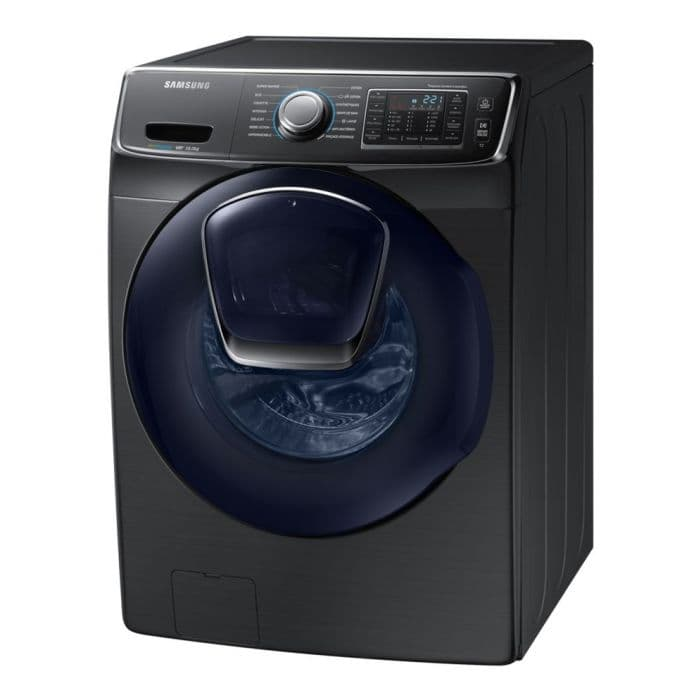
\includegraphics[height=0.9\textwidth]{images/machine.jpg}
    \end{column} 

  \end{columns}
\end{frame}

\section{Différences entre la logique floue et logique classique}

\begin{frame}{Différences entre la logique floue et logique classique}
  C’est sur le principe de la logique classique que fonctionne les ordinateur et
  la plupart des machines numériques. En logique classique, les décisions sont
  binaires : soient vraies ou fausses. C’est sur ce point que la logique floue 
  va se distinguer de la logique classique. En logique floue une décision peut
  être à la fois vraie et fausse en même temps, avec un certain degré
  d'appartenance.
\end{frame}

\begin{frame}
   \begin{block}{Exemple}
    Si l'objet est à moins de 20 mètres, alors il est proche \newline
    Si l'objet est à plus de 20 mètres, alors il est loin
   \end{block}
   En logique floue, un fait n'a plus une appartenance
   stricte à une croyance, mais une appartenance "floue".
   \begin{center}
     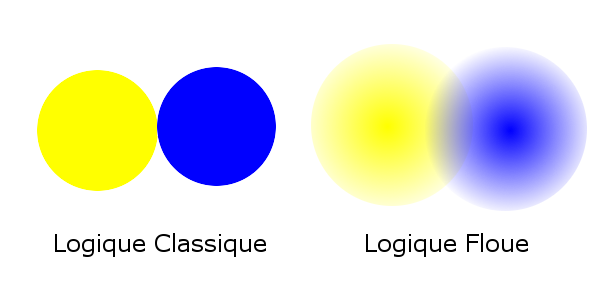
\includegraphics[height=0.4\textwidth]{images/logique_floue.png}
   \end{center}
\end{frame}

\section{Le fonctionnement d’un système flou}

\begin{frame}
  Un système flou a pour fonction de calculer des paramètres de sorties en
  fournissant au système un ensemble de règles formulés en langage naturel
  en utilisant les données de capteurs et les règles d’inférence.
\end{frame}

\subsection{La fuzzification}

\begin{frame}{La fuzzification}
  La fuzzification permet de traduire les données numériques provenant
  d’un capteur en variables linguistique. Avec une fonction d’appartenance
  créer par le concepteur du système flou, le système transforme une donnée
  capteur quantitative en variable linguistique qualitative.
\end{frame}
\begin{frame}
  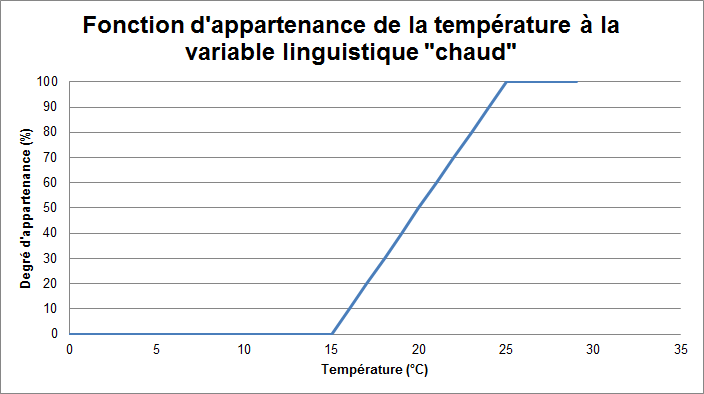
\includegraphics[height=0.5\textwidth]{images/chaud.png}
\end{frame}
\subsection{Le moteur d'inférence}
\begin{frame}{Le moteur d'inférence}
  Le moteur d’inférence prend les variables linguistiques pour
  appliquer les règles d’inférence. Les règles d’inférence sont 
  prédéfinies par le concepteur du système flou. \newline
  Une règle est sous la forme Si condition, alors conclusion:
  \begin{block}{Exemple}
    \begin{itemize}
      \item Si le poids est légés alors vitesse d’essorage faible.
      \item Si les taches sont fortes et grasses, alors le temps de lavage est long.
    \end{itemize}
  \end{block}
\end{frame}
\subsection{La défuzzification}
\begin{frame}{La défuzzification}
  C’est l’étape qui permet de fusionner les différentes commandes générées par
  le moteur d'inférence pour constituer une seule commande de sortie et de
  transformer cette variable linguistique de sortie en donnée numérique.
\end{frame}
\section{Les domaines d’application de la logique floue}
\begin{frame}
  Les domaines d'applications de la logique floue sont très nombreux. On la retrouve :
  \begin{itemize}
    \item En automatique, pour faire de la commande et de la régulation floue, etc.
    \item En traitement du signal, pour faire de la fusion de données, de la classification, de la reconnaissance de forme ou de la recherche d'information, etc.
    \item En robotique, pour faire de la planification de trajectoire, etc.
    \item En traitement d'image, pour atténuer le bruit d'une image, pour faire de l’interpolation, etc.
    \item etc.
  \end{itemize}
\end{frame}

\begin{frame}
  On retrouve la logique floue dans de nombreux secteurs d'activités :
  \begin{itemize}
    \item Médecine (aide au diagnostique, guidage de systèmes chirurgicaux (laser chirurgie de l’œil par exemple), etc.)
    \item Contrôle aérien
    \item Gestions des feux de circulations
    \item Assurances et finances (préventions des risques, aide à la décision)
    \item Environnement (météo, etc.)
    \item Robotique (freins ABS, machines à laver, etc.)
    \item etc.
  \end{itemize}
\end{frame}
\section{Les avantages et inconvénient de la logique floue}
\section{Conclusion}

\end{document}
